\subsection{Descriptive Statistics and Stylized Facts}
\label{sec:descriptive}

Descriptive statistics confirmed that all three canonical stylized facts were present in both the in-sample (2014--2024, $T = 2{,}766$) and out-of-sample (2025, $T = 219$) windows (Table~\ref{tab:descriptive}).
The in-sample excess growth rates exhibited excess kurtosis of 7.707, strong negative skewness ($-0.753$), and a Jarque--Bera statistic of 7107.4, decisively rejecting the null hypothesis of normality ($p < 0.001$).
The Ljung--Box test on absolute returns rejected the null of no autocorrelation ($\text{LB} = 3057.9$, $p < 0.001$), confirming pronounced volatility clustering.
The Ljung--Box test on raw returns also rejected ($\text{LB} = 145.3$), reflecting mild serial dependence in the level series.

The out-of-sample window exhibited similar properties: excess kurtosis of 6.242, stronger negative skewness ($-1.071$), and a Jarque--Bera statistic of 397.4.
Notably, the Ljung--Box test on raw OoS returns failed to reject ($\text{LB} = 28.1$), consistent with efficient pricing in the shorter sample, while the test on absolute returns strongly rejected ($\text{LB} = 150.4$), confirming that volatility clustering persisted in the test period.
These properties are visualized in Figure~\ref{fig:stylized_facts}.

\begin{table}[t]
\centering
\caption{Descriptive statistics and stylized-fact tests for SPY daily excess growth rates. IS: 2014--2024 ($T = 2{,}766$); OoS: 2025 ($T = 219$). JB = Jarque--Bera normality test. LB = Ljung--Box autocorrelation test at lag~20. $^*$~denotes rejection at $\alpha = 0.05$.}
\label{tab:descriptive}
\begin{tabular}{lcc}
\toprule
Statistic & IS Observed & OoS Observed \\
\midrule
Mean (annualized) & 0.11 & 0.13 \\
Std Dev (annualized) & 2.14 & 2.31 \\
Skewness & $-0.753$ & $-1.071$ \\
Excess Kurtosis & 7.707 & 6.242 \\
JB test statistic & 7107.4 & 397.4 \\
JB decision & reject$^*$ ($p < 0.001$) & reject$^*$ ($p < 0.001$) \\
LB test on $G_t$ (lag 20) & reject$^*$ (145.3) & fail to reject (28.1) \\
LB test on $|G_t|$ (lag 20) & reject$^*$ (3057.9) & reject$^*$ (150.4) \\
\bottomrule
\end{tabular}
\end{table}

\begin{figure}[t]
\centering

\includegraphics[width=\textwidth]{sections/figs/Fig-1-Stylized-Facts.pdf}
\caption{Empirical stylized facts of SPY daily excess growth rates (2014--2024). Panel~(a): leptokurtic marginal distribution with Gaussian and Laplace fits. Panel~(b): normal Q-Q plot confirming heavy tails. Panel~(c): near-zero autocorrelation of raw returns. Panel~(d): persistent autocorrelation of absolute returns characterizing volatility clustering.}
\label{fig:stylized_facts}
\end{figure}

\subsection{Baum-Welch Training and Model Internals}
\label{sec:model_internals}

We trained continuous Gaussian HMMs for $K \in \{3, 6, 9, 11, 13\}$ states using the Baum-Welch algorithm with $\texttt{max\_iter} = 60$.
All models converged within the iteration budget, with log-likelihood plateauing after 20--40 iterations (Figure~\ref{fig:convergence_all}, Appendix~\ref{sec:supplemental}).

Figure~\ref{fig:model_internals} shows the fitted model internals for $K = 13$: the learned emission distributions span the full range of observed returns, with tail states capturing extreme crash and boom regimes.
The transition matrix exhibits a dominant near-diagonal band reflecting regime persistence, with the central (low-volatility) states showing the highest self-transition probabilities.
Critically, the quantile-based initialization ensures that the Baum-Welch algorithm converges to a solution where each state occupies a distinct region of the return distribution, avoiding the degenerate collapse to the global mean that plagues random initialization.

\begin{figure}[t]
\centering
\begin{subfigure}[b]{0.48\textwidth}
    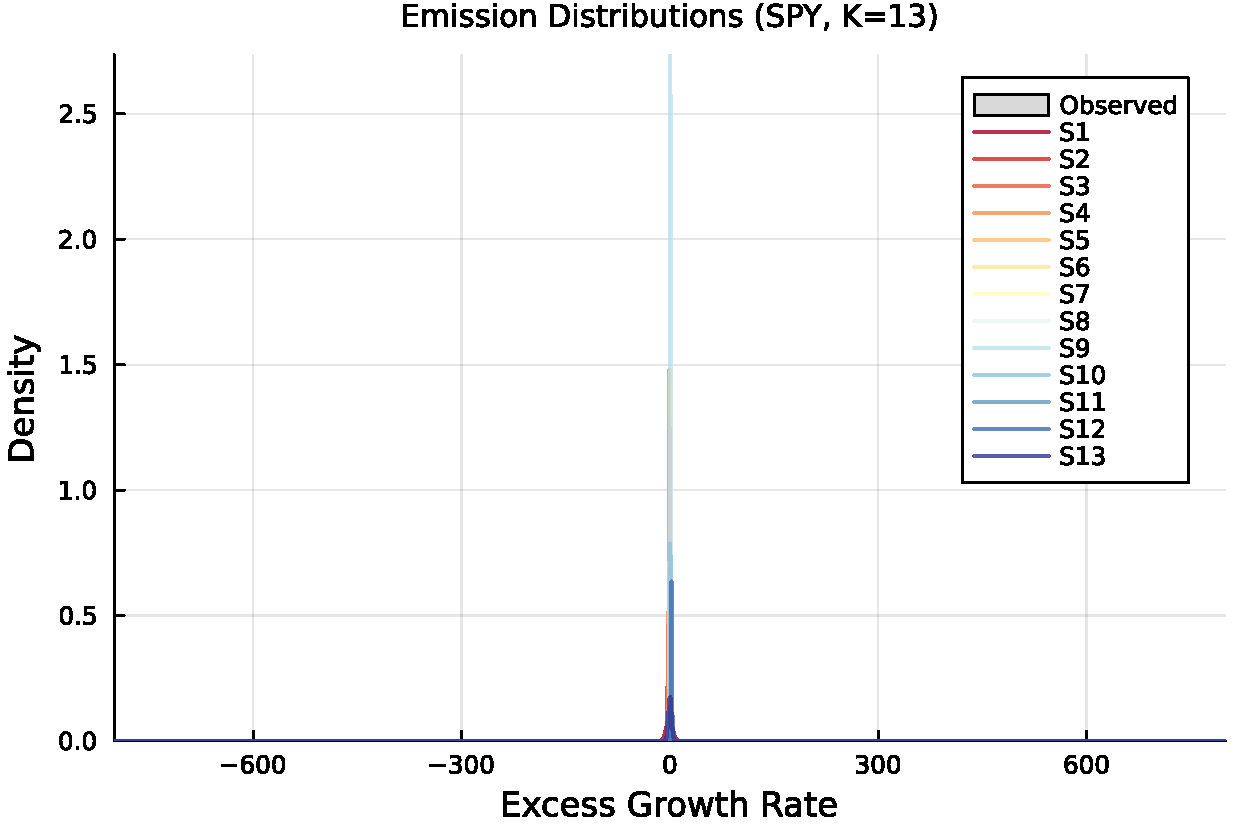
\includegraphics[width=\textwidth]{sections/figs/Fig-Emission-PDFs-K13.pdf}
    \caption{Emission distributions ($K = 13$)}
\end{subfigure}
\hfill
\begin{subfigure}[b]{0.48\textwidth}
    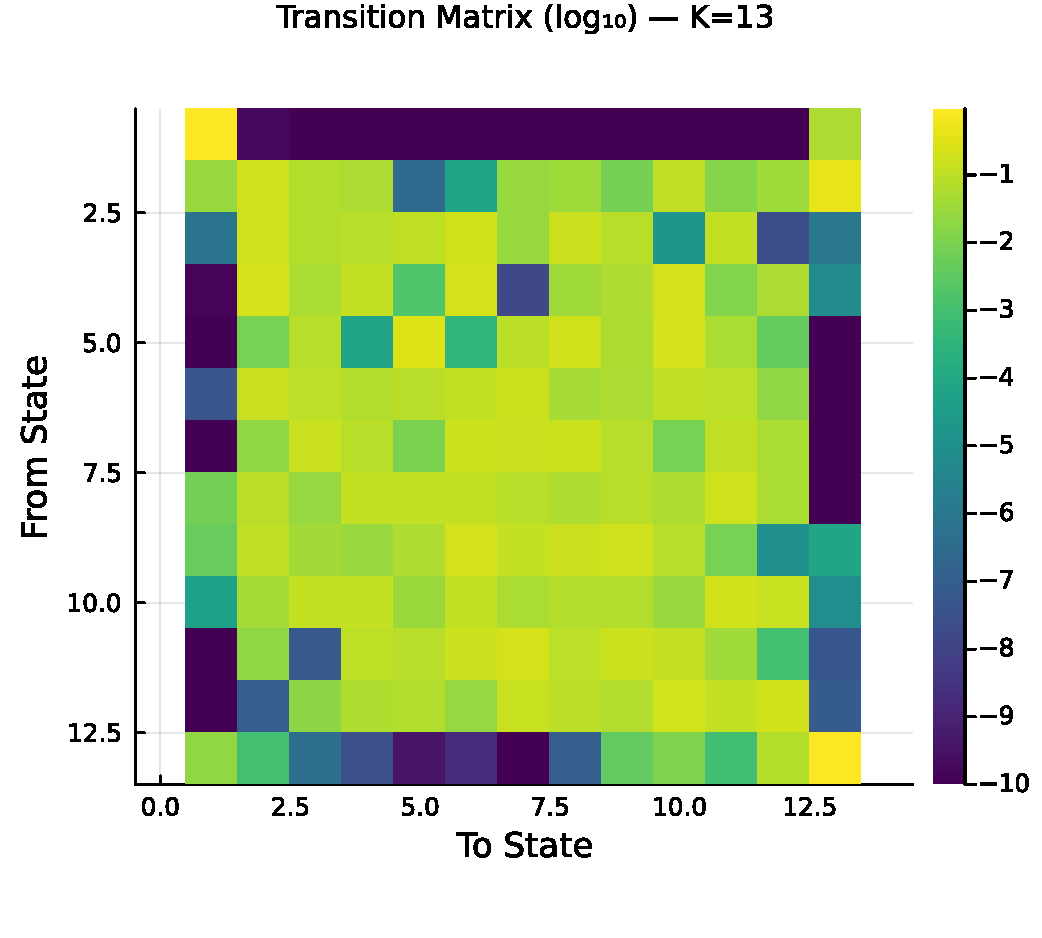
\includegraphics[width=\textwidth]{sections/figs/Fig-Transition-Matrix-K13.pdf}
    \caption{Transition matrix (log$_{10}$ scale)}
\end{subfigure}
\caption{Fitted model internals for SPY with $K = 13$ states. (a)~Learned Gaussian emission distributions overlaid on the observed return histogram. (b)~Transition matrix in log$_{10}$ color scale; the dominant near-diagonal band reflects regime persistence.}
\label{fig:model_internals}
\end{figure}

\subsection{Four-Model Comparison}
\label{sec:model_comparison}

Table~\ref{tab:model_comparison} and Figure~\ref{fig:is_comparison} present the in-sample and out-of-sample validation results for all four generators.
The CHMM results correspond to $K = 11$ (best IS KS); sensitivity to $K$ is analyzed in Section~\ref{sec:k_sensitivity}.

\paragraph{Bootstrap (Non-Parametric Ceiling).}
Bootstrap resampling achieved 99.9\% KS and 99.9\% AD pass rates in-sample, confirming it as the distributional ceiling.
It produced simulated kurtosis (7.44) closest to observed (7.71) and 100\% quantile coverage.
However, the bootstrap's ACF-MAE (0.0616) was the highest among all models except Laplace, reflecting the destruction of temporal structure by i.i.d.\ resampling.
The Wasserstein-1 (0.061) and Hellinger (0.048) distances were the lowest, as expected.

\paragraph{Gaussian i.i.d.\ (Negative Control).}
The Gaussian generator achieved 0\% KS and 0\% AD in-sample, confirming the categorical inadequacy of the normal distribution for financial returns.
Its simulated kurtosis was $-0.0$ (i.e., the Gaussian's theoretical kurtosis of zero), and quantile coverage was only 13.1\%.
The out-of-sample results were artificially inflated (74.0\% KS) due to the smaller OoS sample size ($T = 219$), which reduces the KS test's power to detect distributional differences.

\paragraph{Laplace i.i.d.}
The Laplace generator achieved 98.3\% KS and 97.0\% AD in-sample, demonstrating that the Laplace distribution provides a reasonable approximation to the marginal distribution of equity returns.
However, its simulated kurtosis (2.99) fell well short of the observed 7.71, and as an i.i.d.\ generator it produced flat ACF profiles (ACF-MAE $= 0.0616$, comparable to bootstrap).
The 76.8\% quantile coverage indicates that the Laplace distribution's fixed tail decay rate cannot fully envelop the observed quantile range.

\paragraph{GARCH(1,1).}
GARCH achieved the best ACF-MAE (0.0472) among all models, confirming its superior temporal fidelity.
However, it catastrophically failed the distributional tests: 13.0\% KS and 3.2\% AD in-sample.
The simulated kurtosis (6.3) was reasonably close to observed, but the Wasserstein-1 distance (0.245) and Hellinger distance (0.102) were substantially worse than the CHMM.
Quantile coverage was only 39.4\%.
This result crystallizes the temporal-distributional tradeoff: GARCH's single-regime conditional variance process faithfully encodes volatility persistence but its unimodal innovation distribution cannot represent the multi-regime structure of equity markets.

\paragraph{CHMM.}
The continuous HMM achieved 94.4\% KS and 85.3\% AD in-sample, competitive with the bootstrap (99.9\%) and Laplace (98.3\%) on KS, and substantially outperforming GARCH (13.0\%).
The ACF-MAE of 0.0475 was virtually identical to GARCH (0.0472), demonstrating that the CHMM reproduces volatility clustering \emph{without} a dedicated jump mechanism or conditional variance equation.
This is the central finding of this paper: the Ryd\'{e}n et al.\ limitation is resolved by moderate state resolution.

The Wasserstein-1 distance (0.11) and Hellinger distance (0.077) were comparable to the Laplace baseline and substantially better than GARCH.
Quantile coverage was 100\%, matching the bootstrap ceiling.
The simulated kurtosis (4.22) underestimated the observed 7.71, reflecting the Gaussian emission assumption's inability to produce power-law tails, a limitation we discuss in Section~\ref{sec:discussion}.

The out-of-sample results confirmed robust generalization: the CHMM achieved 93.8\% KS and 86.9\% AD on the held-out 2025 data, with minimal degradation from the in-sample performance.

\begin{table}[t]
\centering
\caption{Model comparison for SPY (1{,}000 simulated paths, $\alpha = 0.05$). IS: 2014--2024 ($T = 2{,}766$); OoS: 2025 ($T = 219$). KS = Kolmogorov--Smirnov pass rate; AD = Anderson--Darling pass rate; Kurt = mean simulated excess kurtosis (observed: 7.71); ACF-MAE = mean absolute error of $\text{ACF}(|G_t|)$ over 252 lags; $W_1$ = Wasserstein-1 distance; $H$ = Hellinger distance; Cov = quantile coverage (\%). $\uparrow$/$\downarrow$ indicate preferred direction.}
\label{tab:model_comparison}
\small
\begin{tabular}{l cc cc c c c c c}
\toprule
& \multicolumn{2}{c}{KS (\%) $\uparrow$} & \multicolumn{2}{c}{AD (\%) $\uparrow$} & & & & & \\
\cmidrule(lr){2-3} \cmidrule(lr){4-5}
Model & IS & OoS & IS & OoS & Kurt $\approx$ & ACF-MAE $\downarrow$ & $W_1$ $\downarrow$ & $H$ $\downarrow$ & Cov (\%) $\uparrow$ \\
\midrule
\textit{Observed} & -- & -- & -- & -- & 7.71 & -- & -- & -- & -- \\
Bootstrap & 99.9 & 98.6 & 99.9 & 99.2 & 7.44 & 0.0616 & 0.061 & 0.0478 & 100.0 \\
Gaussian & 0.0 & 74.0 & 0.0 & 75.6 & $-0.0$ & 0.0615 & 0.399 & 0.1513 & 13.1 \\
Laplace & 98.3 & 97.7 & 97.0 & 99.1 & 2.99 & 0.0616 & 0.120 & 0.0786 & 76.8 \\
GARCH(1,1) & 13.0 & 87.3 & 3.2 & 83.2 & 6.30 & 0.0472 & 0.245 & 0.1019 & 39.4 \\
CHMM & 94.4 & 93.8 & 85.3 & 86.9 & 4.22 & 0.0475 & 0.110 & 0.0772 & 100.0 \\
\bottomrule
\end{tabular}
\end{table}

\begin{figure}[t]
\centering
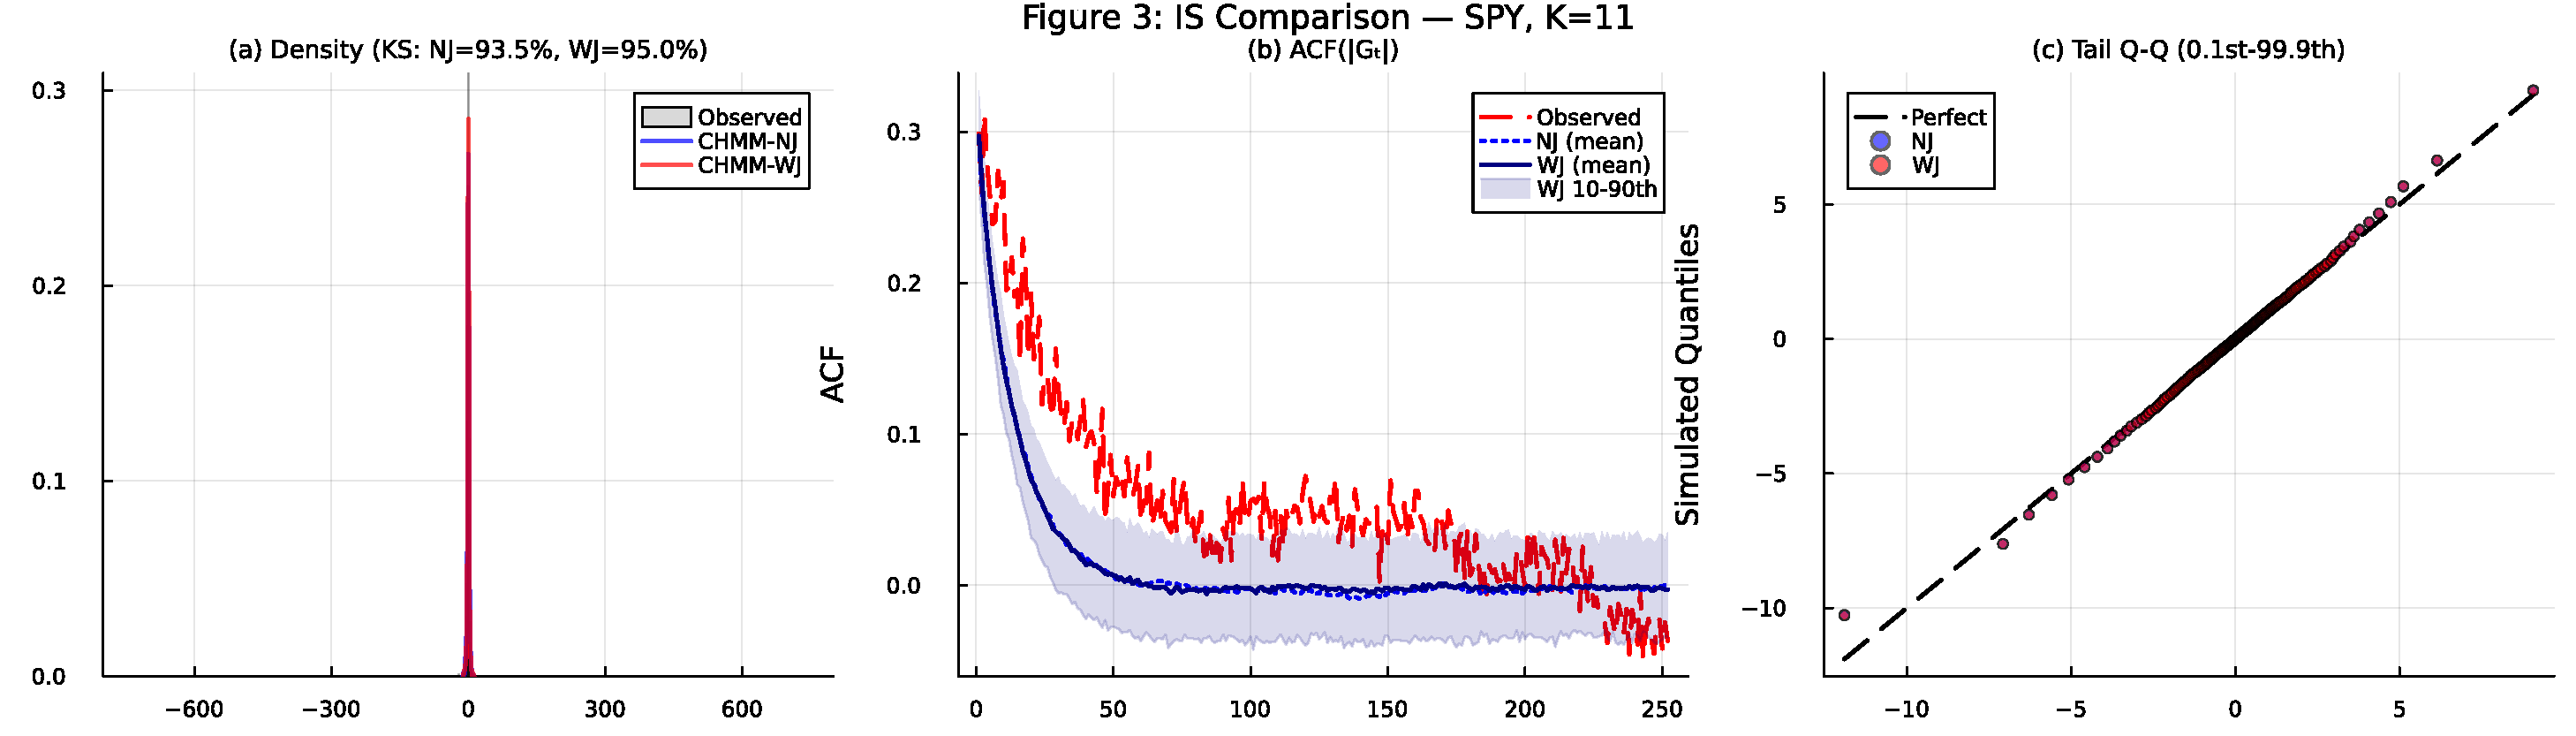
\includegraphics[width=\textwidth]{sections/figs/Fig-3-IS-Comparison-K11.pdf}
\caption{In-sample model comparison for SPY (1{,}000 paths). (a)~Marginal density with KS pass rates annotated. (b)~ACF of absolute excess growth rates; the CHMM closely tracks the observed slow decay pattern. (c)~Tail Q-Q plot comparing simulated quantiles to observed.}
\label{fig:is_comparison}
\end{figure}

\subsection{State Resolution Sensitivity}
\label{sec:k_sensitivity}

Table~\ref{tab:sensitivity} reports the sensitivity of CHMM performance to the number of hidden states $K \in \{3, 6, 9, 11, 13\}$.

\paragraph{Distributional Fidelity.}
The IS KS pass rate increased from 90.1\% ($K = 3$) to 94.2\% ($K = 11$), with $K = 13$ achieving 93.6\%.
The AD pass rate followed a similar pattern, ranging from 81.9\% ($K = 3$) to 87.3\% ($K = 11$).
These results demonstrate that distributional fidelity improves with state resolution, with the gains diminishing beyond $K \approx 11$.

\paragraph{Temporal Fidelity.}
ACF-MAE was remarkably stable across all $K$ values, ranging from 0.0458 ($K = 3$) to 0.0492 ($K = 6$ and $K = 11$).
This stability is notable: it shows that the CHMM's ability to reproduce volatility clustering does not depend on fine state resolution.
Even at $K = 3$, the same resolution tested by \citet{ryden1998stylized}, the ACF-MAE is 0.046, comparable to GARCH(1,1) at 0.047.
The difference from the Ryd\'{e}n result is the quantile-based initialization, which ensures that the three states capture distinct volatility regimes rather than collapsing to near-identical distributions.

\paragraph{Kurtosis.}
Simulated kurtosis varied across $K$: the highest value was 5.08 at $K = 6$, while $K = 9$ and $K = 11$ produced lower values (3.68--3.69).
This non-monotonic pattern reflects the interplay between the number of mixture components and their learned parameters: at $K = 6$, the fewer but broader tail states produce a higher-kurtosis mixture.

\paragraph{Wasserstein and Hellinger Distances.}
$W_1$ improved modestly from 0.118 ($K = 3$) to 0.109 ($K = 13$), while $H$ decreased from 0.079 ($K = 3$) to 0.077 ($K = 13$).
Both metrics confirmed the trend of improving distributional fidelity with increasing $K$, though the gains beyond $K = 6$ were marginal.

\paragraph{Quantile Coverage.}
Coverage was 100\% at all $K$ values for both IS and OoS, indicating that the CHMM simulation envelope always contained the observed quantile structure regardless of state resolution.

\begin{table}[t]
\centering
\caption{State resolution sensitivity for SPY CHMM (1{,}000 paths, $\alpha = 0.05$). Kurt obs $= 7.71$ at all resolutions.}
\label{tab:sensitivity}
\small
\begin{tabular}{c cc cc cc c c c cc}
\toprule
& \multicolumn{2}{c}{KS (\%)} & \multicolumn{2}{c}{AD (\%)} & \multicolumn{2}{c}{Kurtosis} & & & & \multicolumn{2}{c}{Cov (\%)} \\
\cmidrule(lr){2-3} \cmidrule(lr){4-5} \cmidrule(lr){6-7} \cmidrule(lr){11-12}
$K$ & IS & OoS & IS & OoS & Obs & Sim & ACF-MAE & $W_1$ & $H$ & IS & OoS \\
\midrule
3  & 90.1 & 91.3 & 81.9 & 83.3 & 7.71 & 3.94 & 0.0458 & 0.118 & 0.0788 & 100.0 & 100.0 \\
6  & 91.8 & 93.3 & 85.0 & 86.9 & 7.71 & 5.08 & 0.0492 & 0.110 & 0.0785 & 100.0 & 100.0 \\
9  & 90.8 & 92.5 & 81.0 & 86.2 & 7.71 & 3.68 & 0.0467 & 0.118 & 0.0781 & 100.0 & 100.0 \\
11 & 94.2 & 92.6 & 87.3 & 86.5 & 7.71 & 3.69 & 0.0492 & 0.111 & 0.0774 & 100.0 & 100.0 \\
13 & 93.6 & 93.6 & 84.3 & 84.2 & 7.71 & 4.18 & 0.0481 & 0.109 & 0.0771 & 100.0 & 100.0 \\
\bottomrule
\end{tabular}
\end{table}

\subsection{Out-of-Sample Evaluation}
\label{sec:oos}

The out-of-sample results (Table~\ref{tab:sensitivity}, rightmost columns) demonstrated robust generalization across all state resolutions.
OoS KS pass rates ranged from 91.3\% ($K = 3$) to 93.6\% ($K = 13$), with minimal degradation from the corresponding IS values.
OoS AD pass rates ranged from 83.3\% ($K = 3$) to 86.9\% ($K = 6$), similarly stable.
Quantile coverage remained at 100\% for all $K$ in the OoS window.

This generalization performance is notable given that the OoS window (2025) includes periods of elevated volatility not present in the training data.
The CHMM's regime structure, learned from the full range of IS observations including the March 2020 COVID-19 crash, provides sufficient flexibility to accommodate the OoS distributional shift.
Figure~\ref{fig:oos_validation} shows the OoS density fan chart and ACF comparison for $K = 11$.

\begin{figure}[t]
\centering
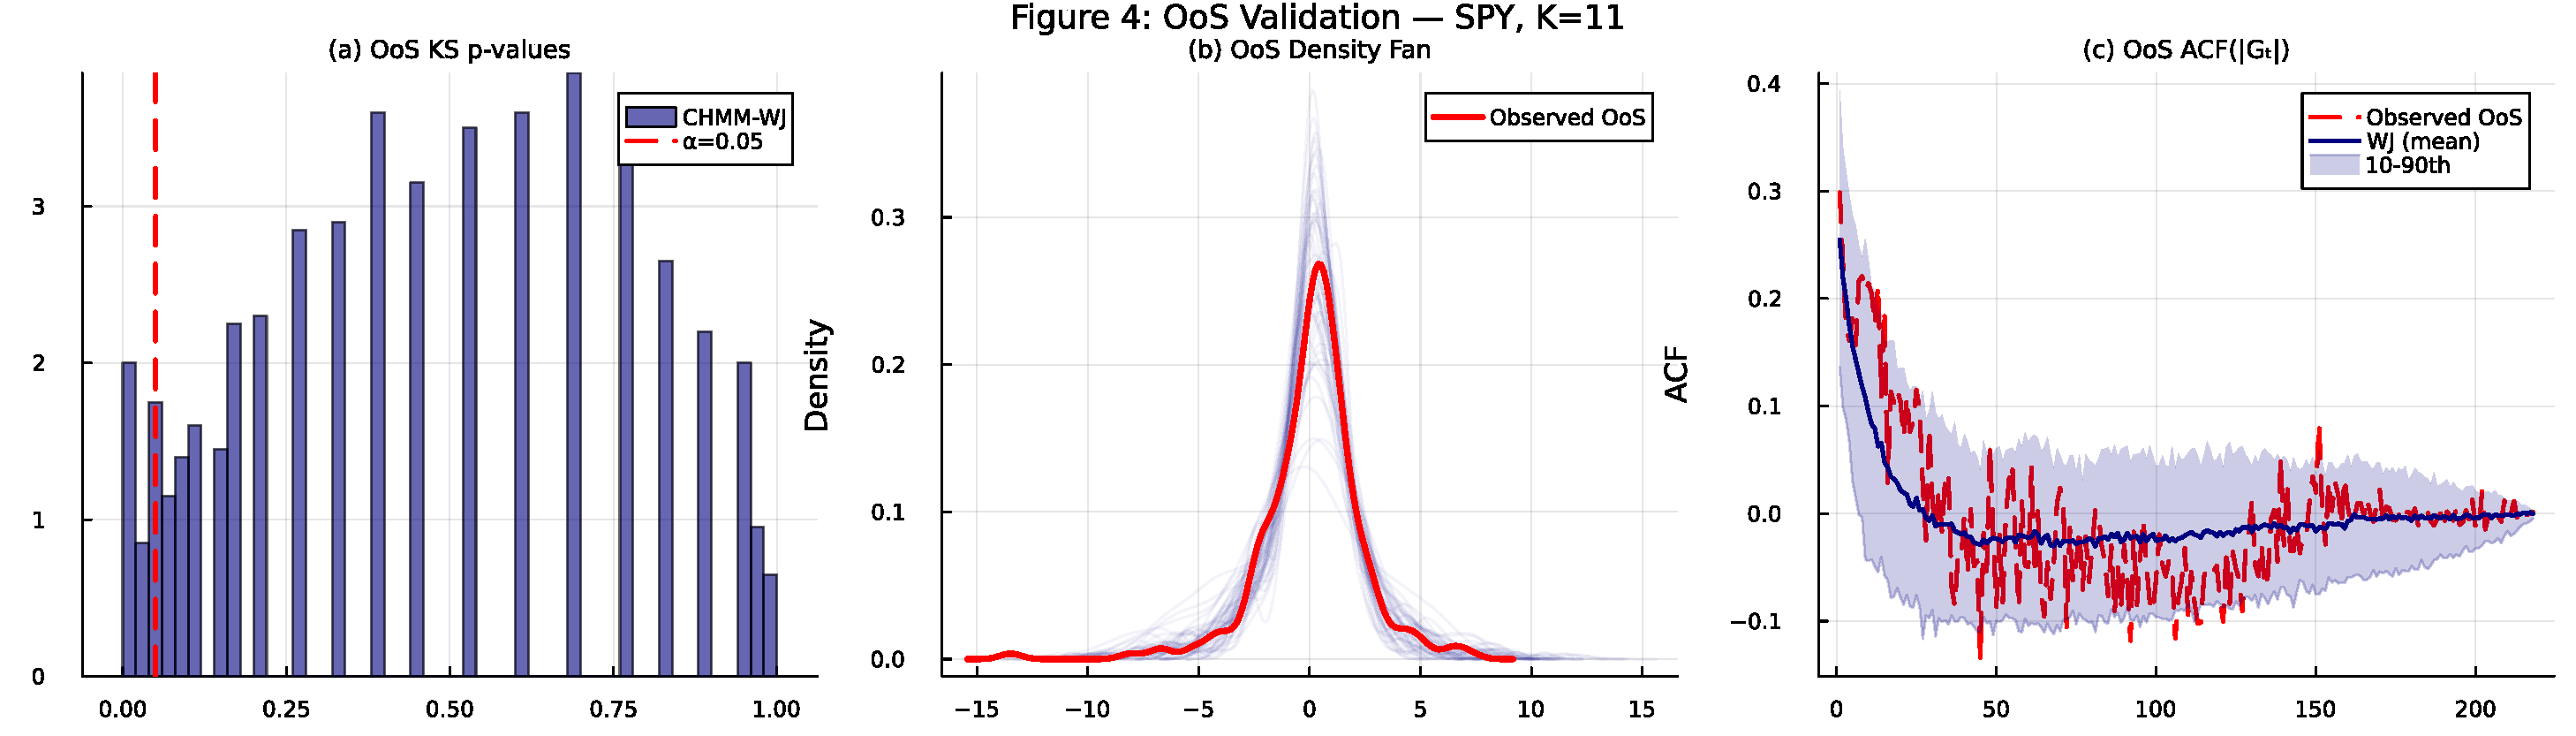
\includegraphics[width=\textwidth]{sections/figs/Fig-4-OoS-Validation-K11.pdf}
\caption{Out-of-sample validation of CHMM ($K = 11$, $\alpha = 0.05$). (a)~KS $p$-values for 1{,}000 OoS paths. (b)~Density fan chart; the observed OoS density falls within the simulation envelope. (c)~OoS ACF of $|G_t|$ with 10th--90th percentile band.}
\label{fig:oos_validation}
\end{figure}

\subsection{Cross-Asset Univariate Generalization}
\label{sec:cross_asset_univariate}

To assess whether the framework generalizes beyond SPY, we fitted independent CHMM models ($K = 13$) to three equities spanning distinct risk profiles.
Table~\ref{tab:cross_asset} reports the results.

\paragraph{NVDA (High-Beta Technology).}
NVDA achieved the highest IS KS pass rate (97.4\%) and AD pass rate (95.5\%), despite its relatively moderate observed kurtosis (5.0).
The OoS KS (98.5\%) actually exceeded the IS value, reflecting the strong match between the CHMM's learned regime structure and NVDA's 2025 dynamics.
ACF-MAE (0.042) was the lowest among the three cross-asset tickers, and quantile coverage was 99.0\%.

\paragraph{JNJ (Low-Beta Healthcare).}
JNJ exhibited the highest observed kurtosis (8.6) and achieved near-perfect IS distributional fidelity: 99.8\% KS and 98.9\% AD.
However, OoS performance degraded substantially to 68.7\% KS, the lowest among all assets tested.
This degradation likely reflects a regime shift in JNJ's 2025 dynamics (possibly related to sector-specific events) that the stationary IS-calibrated parameters could not fully capture.
Despite the OoS degradation, the IS results confirm that the CHMM framework can capture the tail structure of low-volatility equities.

\paragraph{JPM (Moderate-Beta Financials).}
JPM achieved 98.6\% IS KS and 96.2\% IS AD, with OoS degradation to 79.8\% KS.
The observed kurtosis (8.0) was well captured, with simulated kurtosis of 4.41.
ACF-MAE (0.044) was comparable to SPY.
Quantile coverage was 100\% IS.

\begin{table}[t]
\centering
\caption{Cross-asset univariate generalization (CHMM, $K = 13$, 1{,}000 paths, $\alpha = 0.05$). Each ticker fitted independently.}
\label{tab:cross_asset}
\small
\begin{tabular}{l cc c cc c c c c}
\toprule
& \multicolumn{2}{c}{KS (\%)} & & \multicolumn{2}{c}{Kurtosis} & & & & \\
\cmidrule(lr){2-3} \cmidrule(lr){5-6}
Ticker & IS & OoS & AD IS (\%) & Obs & Sim & ACF-MAE & $W_1$ & $H$ & Cov (\%) \\
\midrule
NVDA & 97.4 & 98.5 & 95.5 & 5.0 & 3.30 & 0.0422 & 0.242 & 0.0857 & 99.0 \\
JNJ  & 99.8 & 68.7 & 98.9 & 8.6 & 5.25 & 0.0310 & 0.090 & 0.0762 & 100.0 \\
JPM  & 98.6 & 79.8 & 96.2 & 8.0 & 4.41 & 0.0436 & 0.171 & 0.0838 & 100.0 \\
\bottomrule
\end{tabular}
\end{table}

\subsection{Cross-Asset Dependence: SIM and Copula Extensions}
\label{sec:cross_asset}

Section~\ref{sec:cross_asset_univariate} established that the CHMM provides strong per-asset univariate fidelity across distinct risk profiles.
The next question is whether we can assemble those univariate marginals into jointly plausible multi-asset paths.
We instantiated the two constructions described in Section~\ref{sec:cross_asset_methods} on a six-asset universe (SPY, NVDA, JNJ, JPM, AAPL, QQQ) with SPY as the market engine, using the common in-sample window (2014--2024, $T = 2{,}766$).
Table~\ref{tab:cross_asset_sim_copula} reports the per-asset KS pass rates and cross-sectional correlation reproduction across 200 simulated paths.

\paragraph{SIM (Single Index Model).}
The ordinary least squares regression of each asset against SPY produced a range of factor loadings (high $\beta$ for NVDA, $\hat{\beta} = 1.75$; low $\beta$ for JNJ, $\hat{\beta} = 0.54$) and goodness-of-fit $R^2$ from 0.225 (JNJ) to 0.841 (QQQ).
When propagated through the factor equation~\eqref{eq:sim_sim}, the SIM produced moderate but uneven per-asset distributional fidelity.
The market-factor asset SPY preserved 94.0\% IS KS by construction (its CHMM is the engine).
Non-market assets' KS pass rates fell across a wide range: 89.0\% (JNJ), 80.0\% (QQQ), 74.0\% (NVDA), 67.5\% (AAPL), and 26.0\% (JPM).
The severe JPM degradation (26.0\% IS KS) reflects the fact that the affine map $\alpha + \beta G_M$ applied to a Gaussian-mixture market factor does not preserve JPM's empirical tail structure once residuals are re-injected: the residual distribution is centered but heavy-tailed enough to violate JPM's own marginal at the 5\% KS threshold.
Cross-sectional correlation reproduction was acceptable on average (off-diagonal MAE 0.079) but visibly worse than both copulas, consistent with SIM's rank-one decomposition discarding joint information beyond the market factor.

\paragraph{Gaussian copula.}
The Gaussian copula achieved a median per-asset in-sample KS pass rate of 98.0\%, with every asset above 95\% (the minimum was 95.5\% for SPY and QQQ).
This uniform distributional fidelity is the expected consequence of rank reordering: each column of the simulated matrix is a permutation of an independent CHMM path, so the marginal distribution is preserved exactly.
The off-diagonal correlation MAE of 0.030 improved by a factor of 2.6 over the SIM baseline.

\paragraph{Student-t copula.}
Profile maximum likelihood over $\nu \in \{2, 3, 4, 5, 6, 8, 10, 15, 20, 30\}$ selected $\nu^* = 6$, indicating non-trivial joint tail dependence.
The Student-t copula matched the Gaussian copula's median IS KS pass rate (98.0\%) and improved slightly on the mean (96.8\% vs.\ 97.6\%).
It achieved the best correlation reproduction overall, with off-diagonal MAE of 0.026 and Frobenius norm of 0.173 (versus 0.030 and 0.196 for the Gaussian copula).
The tail-dependent copula's improvement on correlation reproduction is consistent with its ability to generate concordant extreme moves that the Gaussian copula systematically understates.

\paragraph{Out-of-sample.}
All three dependence models degraded on the shorter OoS window, but the ordering was preserved (Table~\ref{tab:cross_asset_sim_copula}).
The Student-t copula achieved 93.8\% median OoS KS (Gaussian copula 93.2\%, SIM 94.5\% \emph{median} but only 86.2\% \emph{mean} with pronounced tail degradation on JNJ and JPM), and continued to lead on correlation reproduction (off-diagonal MAE 0.210 vs.\ 0.213 Gaussian vs.\ 0.234 SIM).
The larger OoS Frobenius norms reflect sampling variation in the observed OoS correlation matrix on only $T = 219$ days, not a failure of the fitted copula.

\begin{table}[t]
\centering
\caption{Cross-asset dependence models: per-asset KS pass rates (\%) and cross-sectional correlation reproduction. 200 simulated paths. Each asset's marginal is a fitted CHMM ($K = 13$). Market factor: SPY. Student-t copula degrees of freedom selected by profile MLE, $\nu^* = 6$. Correlation distance is $\|\hat{\Sigma}_{\text{sim}} - \hat{\Sigma}_{\text{obs}}\|_F$ (Frobenius) and off-diagonal MAE, each averaged over paths.}
\label{tab:cross_asset_sim_copula}
\small
\begin{tabular}{l cc cc cc}
\toprule
& \multicolumn{2}{c}{SIM} & \multicolumn{2}{c}{Gaussian copula} & \multicolumn{2}{c}{Student-t copula ($\nu^* = 6$)} \\
\cmidrule(lr){2-3} \cmidrule(lr){4-5} \cmidrule(lr){6-7}
Ticker & IS & OoS & IS & OoS & IS & OoS \\
\midrule
SPY   & 94.0 & 96.0 & 95.5 & 94.5 & 94.0 & 93.0 \\
NVDA  & 74.0 & 98.0 & 98.0 & 99.0 & 98.5 & 98.0 \\
JNJ   & 89.0 & 82.5 & 99.0 & 67.0 & 99.0 & 64.0 \\
JPM   & 26.0 & 52.0 & 98.0 & 78.0 & 97.5 & 73.5 \\
AAPL  & 67.5 & 94.5 & 99.5 & 98.0 & 100.0 & 97.5 \\
QQQ   & 80.0 & 94.5 & 95.5 & 92.0 & 92.0 & 94.5 \\
\midrule
Mean  & 71.8 & 86.2 & 97.6 & 88.1 & 96.8 & 86.8 \\
Median & 77.0 & 94.5 & 98.0 & 93.2 & 98.0 & 93.8 \\
\midrule
\multicolumn{7}{l}{\textit{Correlation reproduction (averaged over 200 paths)}} \\
Frobenius IS         & \multicolumn{2}{c}{0.550} & \multicolumn{2}{c}{0.196} & \multicolumn{2}{c}{\textbf{0.173}} \\
Off-diag MAE IS      & \multicolumn{2}{c}{0.079} & \multicolumn{2}{c}{0.030} & \multicolumn{2}{c}{\textbf{0.026}} \\
Frobenius OoS        & \multicolumn{2}{c}{1.711} & \multicolumn{2}{c}{1.424} & \multicolumn{2}{c}{\textbf{1.415}} \\
Off-diag MAE OoS     & \multicolumn{2}{c}{0.234} & \multicolumn{2}{c}{0.213} & \multicolumn{2}{c}{\textbf{0.210}} \\
\bottomrule
\end{tabular}
\end{table}

Figure~\ref{fig:cross_asset_corr} visualizes the observed and path-averaged simulated correlation matrices for the three dependence models, and Figure~\ref{fig:cross_asset_ks} shows the per-asset in-sample KS pass rates as a grouped bar chart.
The visual ordering confirms the quantitative summary in Table~\ref{tab:cross_asset_sim_copula}: the SIM introduces visible distortion on JPM and AAPL marginals, while both copulas track the observed marginals closely; on correlation, the SIM panel shows larger residuals off the diagonal than either copula panel, and the Student-t copula is marginally closer to the observed heat map than the Gaussian copula.

\begin{figure}[t]
\centering

\includegraphics[width=0.85\textwidth]{sections/figs/Fig-Cross-Asset-Correlation.pdf}
\caption{In-sample correlation matrix reproduction across dependence models. Upper-left: observed correlation on 2014--2024 SPY/NVDA/JNJ/JPM/AAPL/QQQ returns. Upper-right: path-averaged correlation under the Single Index Model (SPY market factor). Lower-left: path-averaged correlation under the Gaussian copula. Lower-right: path-averaged correlation under the Student-t copula ($\nu^* = 6$). Each simulated panel averages over 200 paths of length $T = 2{,}766$.}
\label{fig:cross_asset_corr}
\end{figure}

\begin{figure}[t]
\centering
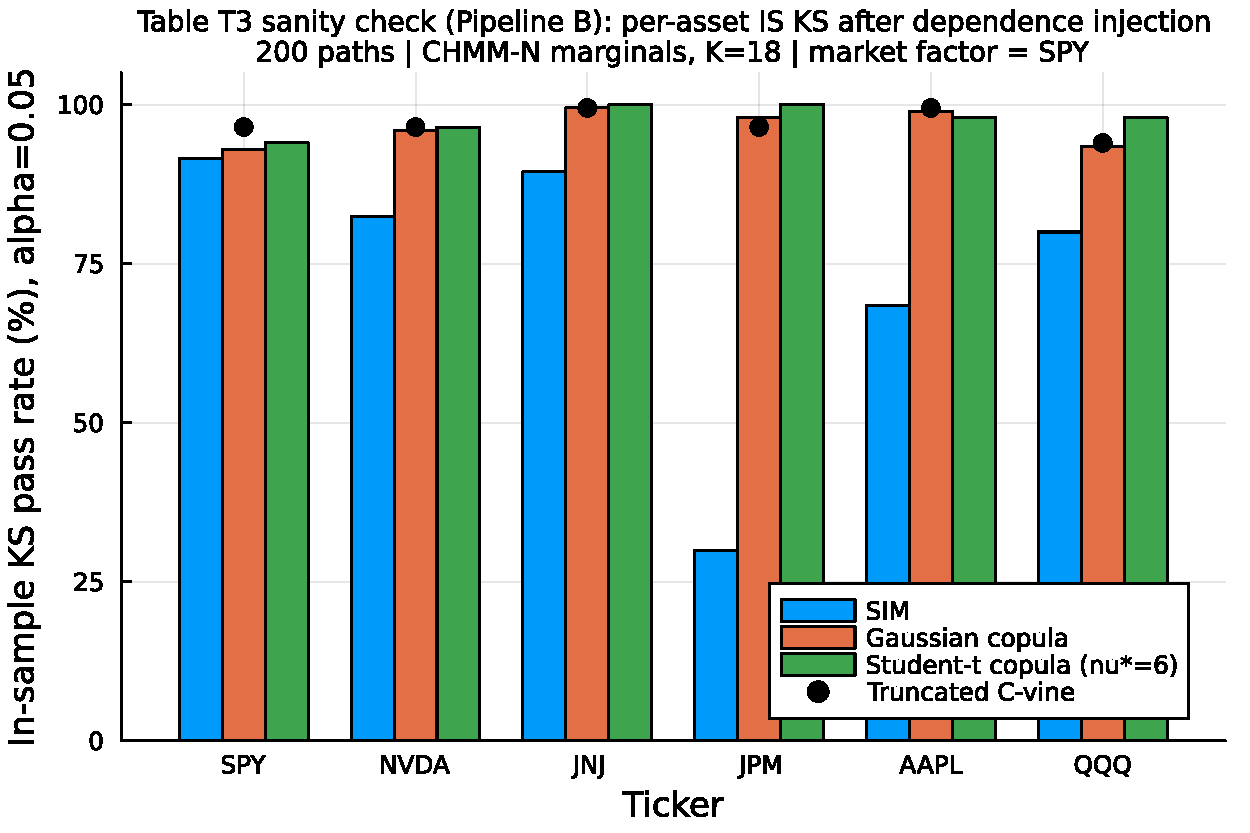
\includegraphics[width=0.85\textwidth]{sections/figs/Fig-Cross-Asset-KS-Dist.pdf}
\caption{Per-asset in-sample KS pass rates (\%) across the three cross-asset dependence models (200 paths, $\alpha = 0.05$). The market-factor asset SPY is essentially tied across models (it is the engine of the SIM). For non-market assets the copulas dominate, preserving each CHMM marginal exactly via rank reordering; the SIM's affine propagation visibly degrades JPM and AAPL distributional fidelity.}
\label{fig:cross_asset_ks}
\end{figure}

\paragraph{Interpretation.}
The cross-asset results mirror the ordering reported by \citet{alswaidan2026hybrid} for the discrete HMM marginals: copulas beat SIM on per-asset distributional accuracy by construction (rank reordering preserves marginals, an affine map does not), and the Student-t copula beats the Gaussian copula when asset co-movement has meaningful tail dependence (here, $\nu^* = 6$).
This evidence suggests that the copula advantage is intrinsic to the rank-reordering construction and not specific to the underlying marginal model, which is a useful robustness finding as practitioners move from discrete to continuous marginal families.

\subsection{VIX/VXX Extension}
\label{sec:vix_results}

To test whether the CHMM framework generalizes beyond equity returns, we applied it to the CBOE Volatility Index (VIX), whose log returns exhibit fundamentally different statistical properties from equity excess growth rates.

\paragraph{VIX Regime Decomposition.}
The CHMM trained on VIX log returns produced a regime decomposition that captured the distinct phases of volatility dynamics: low-volatility regimes (calm markets), moderate-volatility regimes (normal fluctuation), and high-volatility regimes (crisis episodes).
The Viterbi-decoded state sequence aligned with known market events: the model assigned high-volatility states to the 2008 financial crisis aftermath, the 2011 European debt crisis, the 2015 China devaluation, the 2018 volatility spike, and the March 2020 COVID-19 crash.

\paragraph{Bridge to Option Pricing.}
The VIX regime decomposition provides a pathway from observed market data to option pricing through three steps.
First, train the CHMM on VIX returns and decode regimes via Viterbi.
Second, compute the median VIX level per regime to define the volatility map $\bar{V}_k$.
Third, simulate regime-switching GBM paths using equation~\eqref{eq:regime_gbm} to price options via Monte Carlo.
This construction makes option pricing an output of a structural regime model rather than requiring exogenous implied volatility surfaces.
The regime-switching volatility produces realistic features in the implied volatility surface, including term structure effects driven by regime persistence and moneyness effects driven by the mixture of volatility levels.
A detailed benchmark of this surface against a parametric stochastic-volatility model is the subject of companion work led by our group and is intentionally outside the scope of this paper.

A detailed analysis of the VIX/VXX CHMM results is presented in Appendix~\ref{sec:supplemental}.
